\chapter{Performance Evaluation}
\label{chp:perfeval}

Bottleneck can happen in the early time of share mode. The combination of line \ref{alg:l_lts:retdlenough} and \ref{alg:l_lts:retdling} will hold downloading any piece if the uploaded amount is not enough based on the piece we have. Let say we already which piece to download from line \ref{alg:l_lts:dlrare}. In the next round, this piece is not rare anymore. Therefore, we cannot upload this piece. 

\section{Predownload}

\begin{figure}[h]
	\centering
	\includegraphics[width=\textwidth]{pics/results/dpredown_500-12.pdf}
	\caption{Predownload success percentage}
	\label{fig:predownprecent}
\end{figure}

\begin{figure}[h]
	\centering
	\includegraphics[width=\textwidth]{pics/results/hpredown_500-12.pdf}
	\caption{Predownload distributed time}
	\label{fig:predownhist}
\end{figure}

\begin{figure}[h]
	\centering
	\includegraphics[width=\textwidth]{pics/results/tmp_pic_peers-0.png}
	\caption{Amount of peer discovered}
	\label{fig:peeramount}
\end{figure}

\begin{figure}[h]
	\centering
	\includegraphics[width=\textwidth]{pics/results/tmp_pic_peers-1.png}
	\caption{Undetected peer in swarms}
	\label{fig:peer0}
\end{figure}
\todo{From experiment \#46 500 swarm in source. 12h}

% 100 swarm for 12, 24. 500 swarm for 24h
\section{Comparison vs old}
\begin{figure}[t!]
	\begin{adjustwidth}{-2.5cm}{}
		\begin{subfigure}[t]{0.7\textwidth}
			\centering
			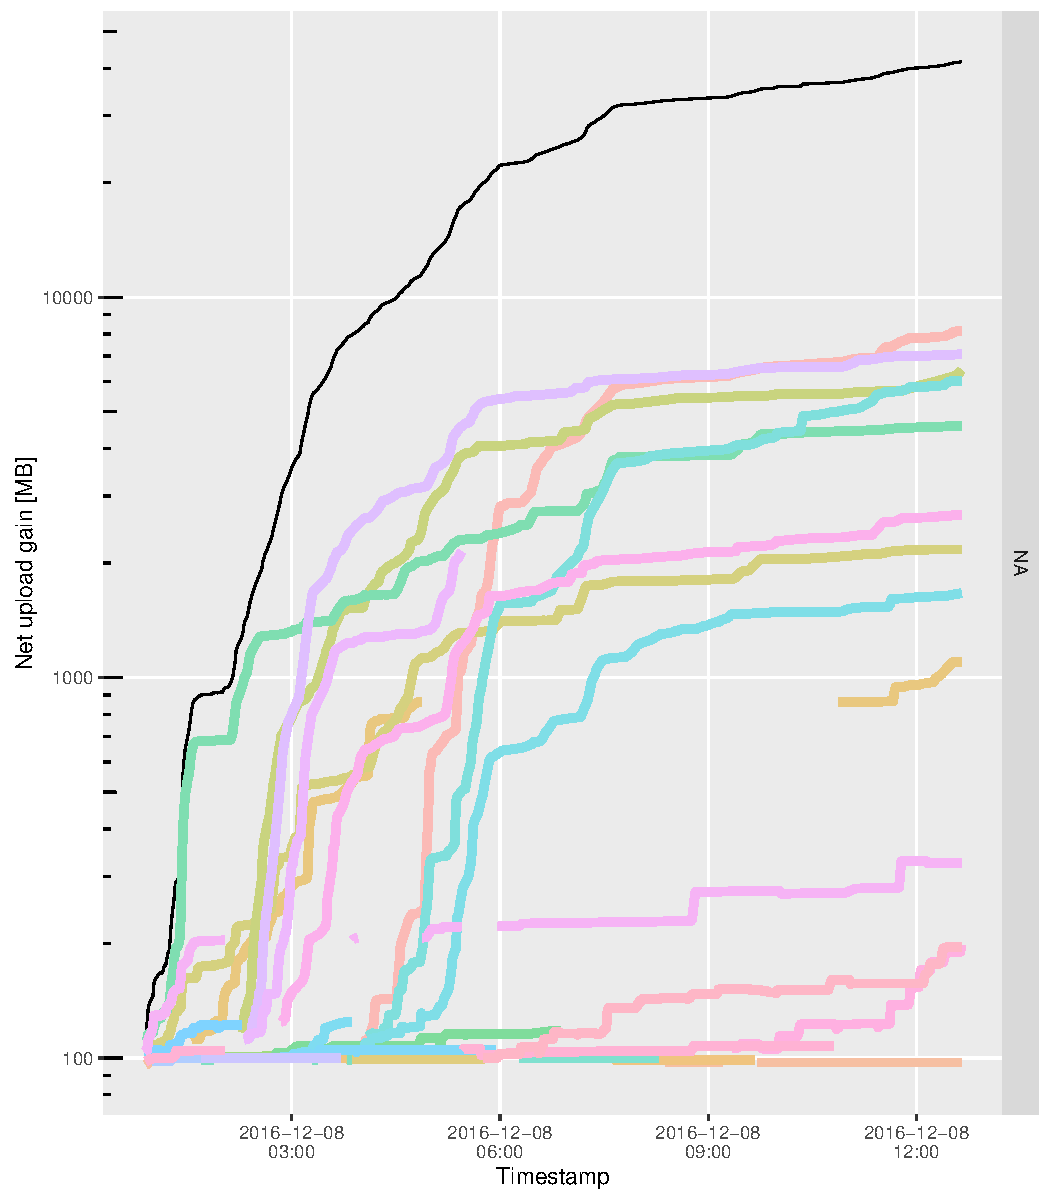
\includegraphics[width=\textwidth]{pics/results/b133.pdf}
			\caption{12 hour new experiment.}
		\end{subfigure}
		~
		\begin{subfigure}[t]{0.7\textwidth}
			\centering
			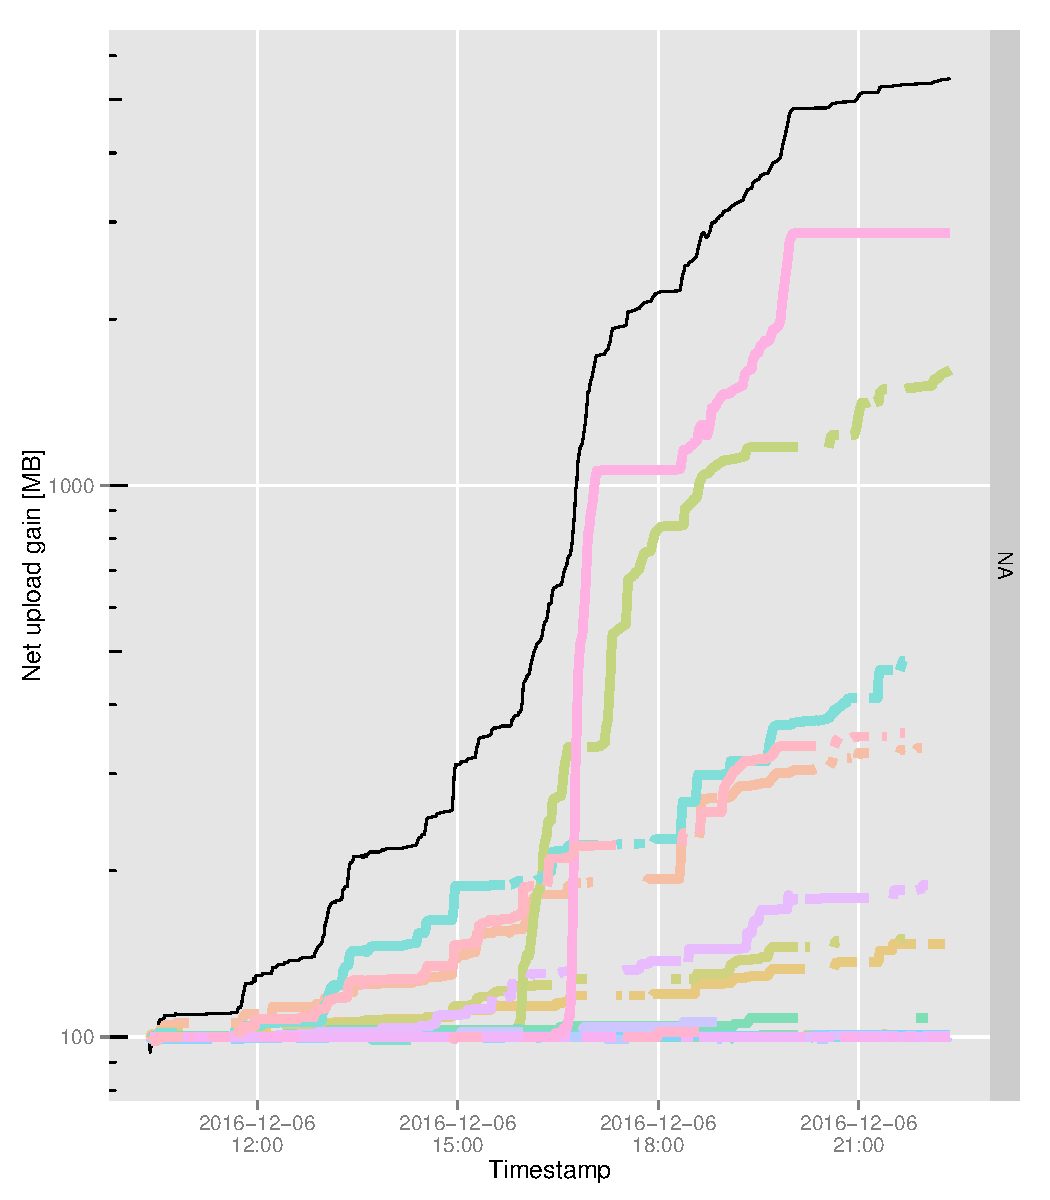
\includegraphics[width=\textwidth]{pics/results/m136.pdf}
			\caption{12 hour old experiment}
		\end{subfigure}
		\caption{New vs old experiments (run separately) result on 12 hour}
	\end{adjustwidth}
\end{figure}

\begin{figure}[t!]
		\begin{adjustwidth}{-2.5cm}{}
	\begin{subfigure}[t]{0.7\textwidth}
		\centering
		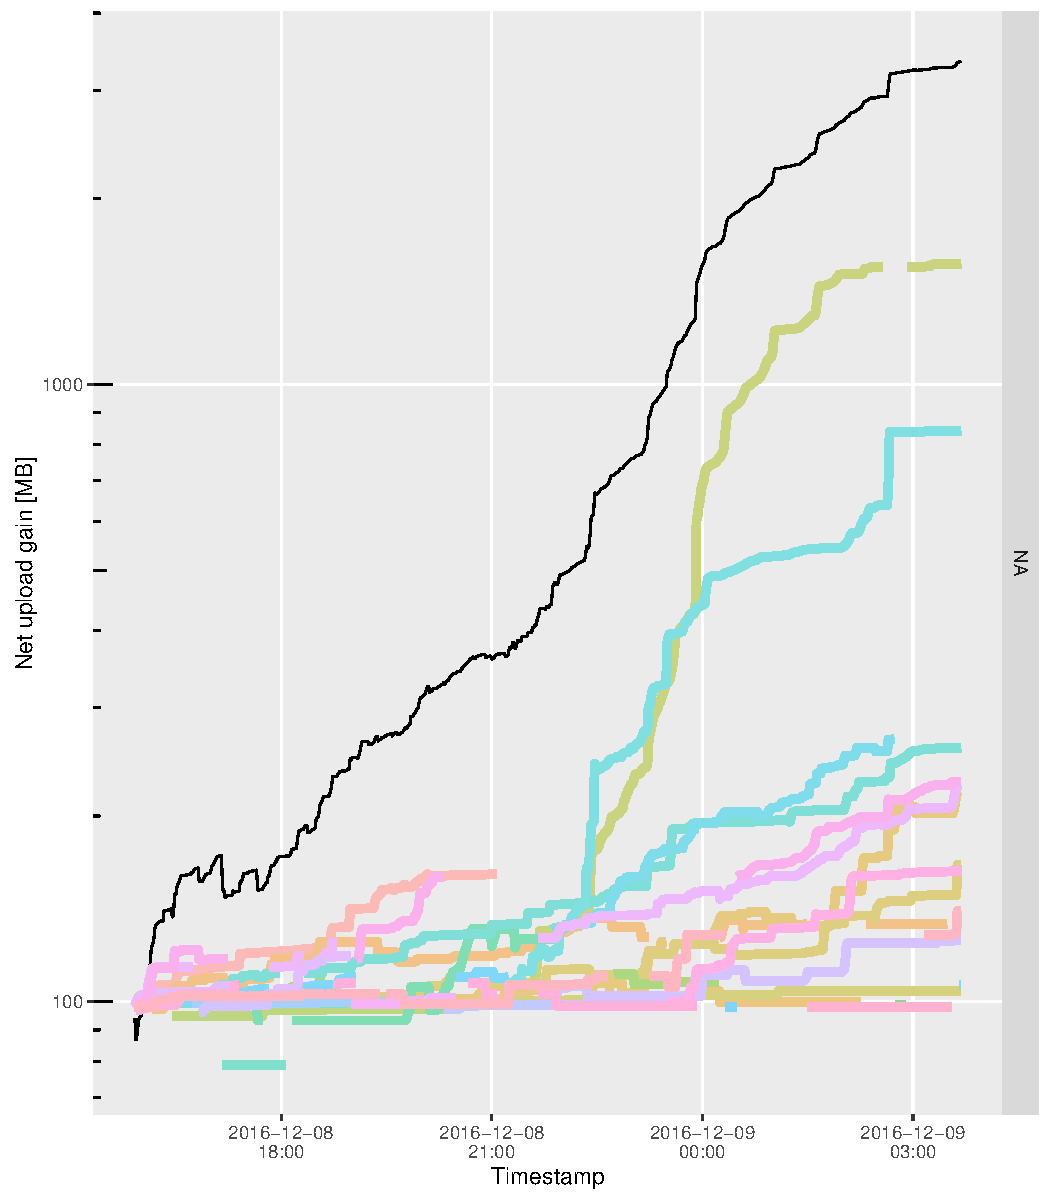
\includegraphics[width=\textwidth]{pics/results/b134.pdf}
		\caption{12 hour new experiment.}
	\end{subfigure}
	~
	\begin{subfigure}[t]{0.7\textwidth}
		\centering
		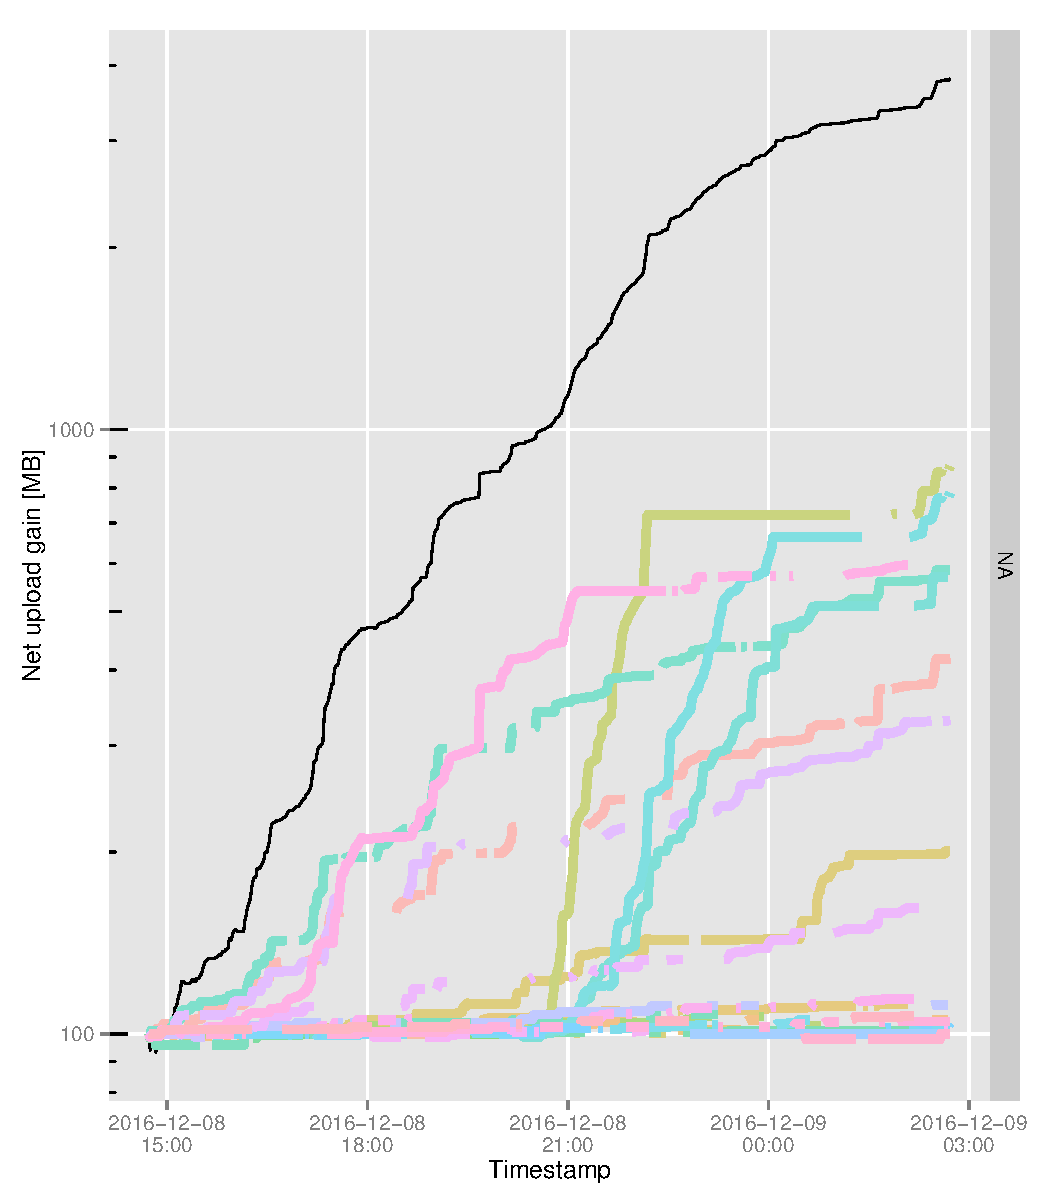
\includegraphics[width=\textwidth]{pics/results/m137.pdf}
		\caption{12 hour old experiment}
	\end{subfigure}
	\caption{New vs old experiments (run in parallel) result on 12 hour}
		\end{adjustwidth}
\end{figure}

\begin{figure}[t!]
	\begin{adjustwidth}{-2.5cm}{}
		\begin{subfigure}[t]{0.7\textwidth}
			\centering
			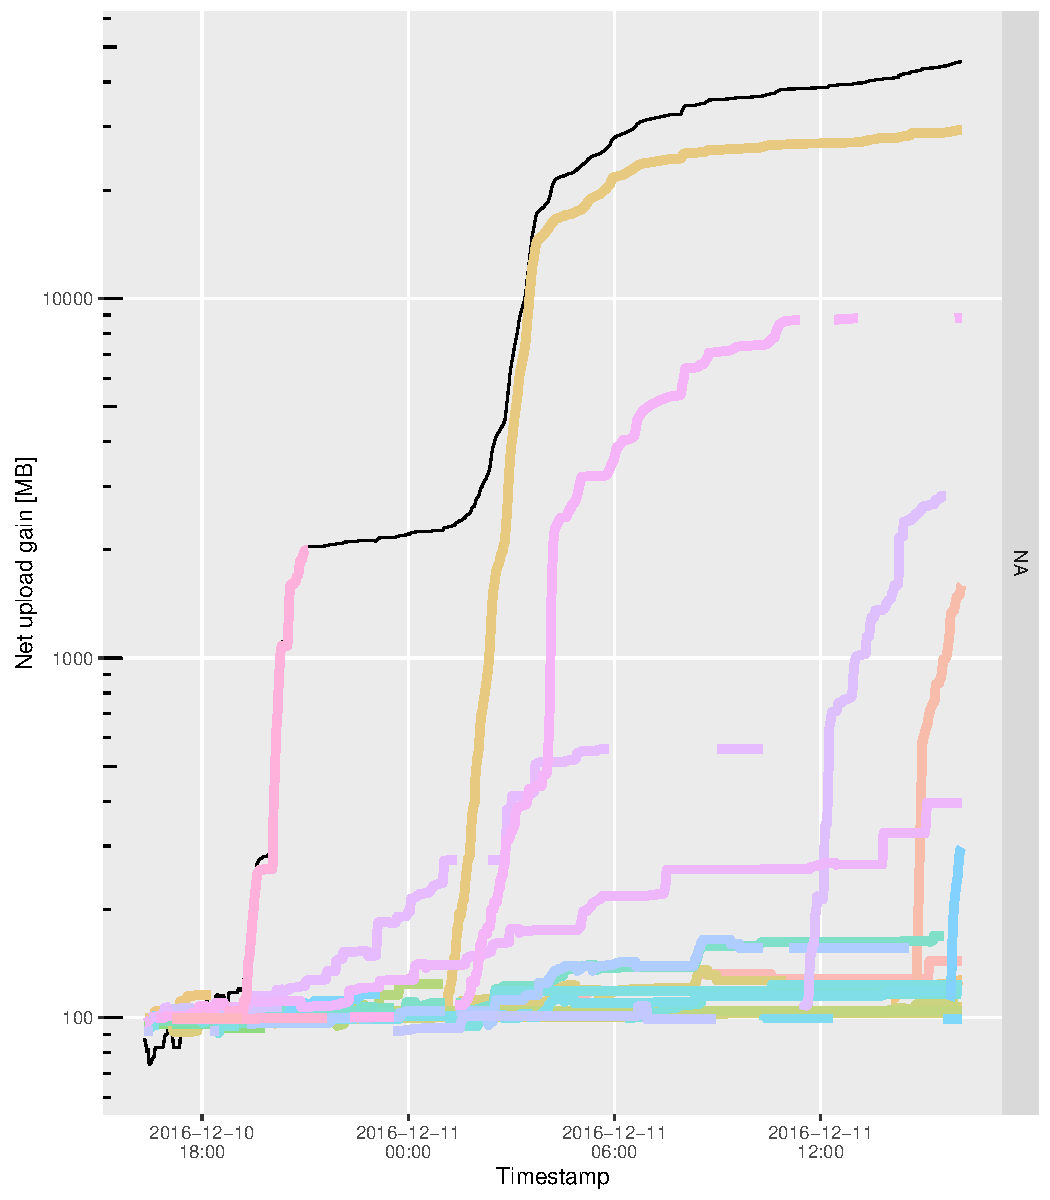
\includegraphics[width=\textwidth]{pics/results/b136.pdf}
			\caption{24 hour new experiment.}
		\end{subfigure}
		~
		\begin{subfigure}[t]{0.7\textwidth}
			\centering
			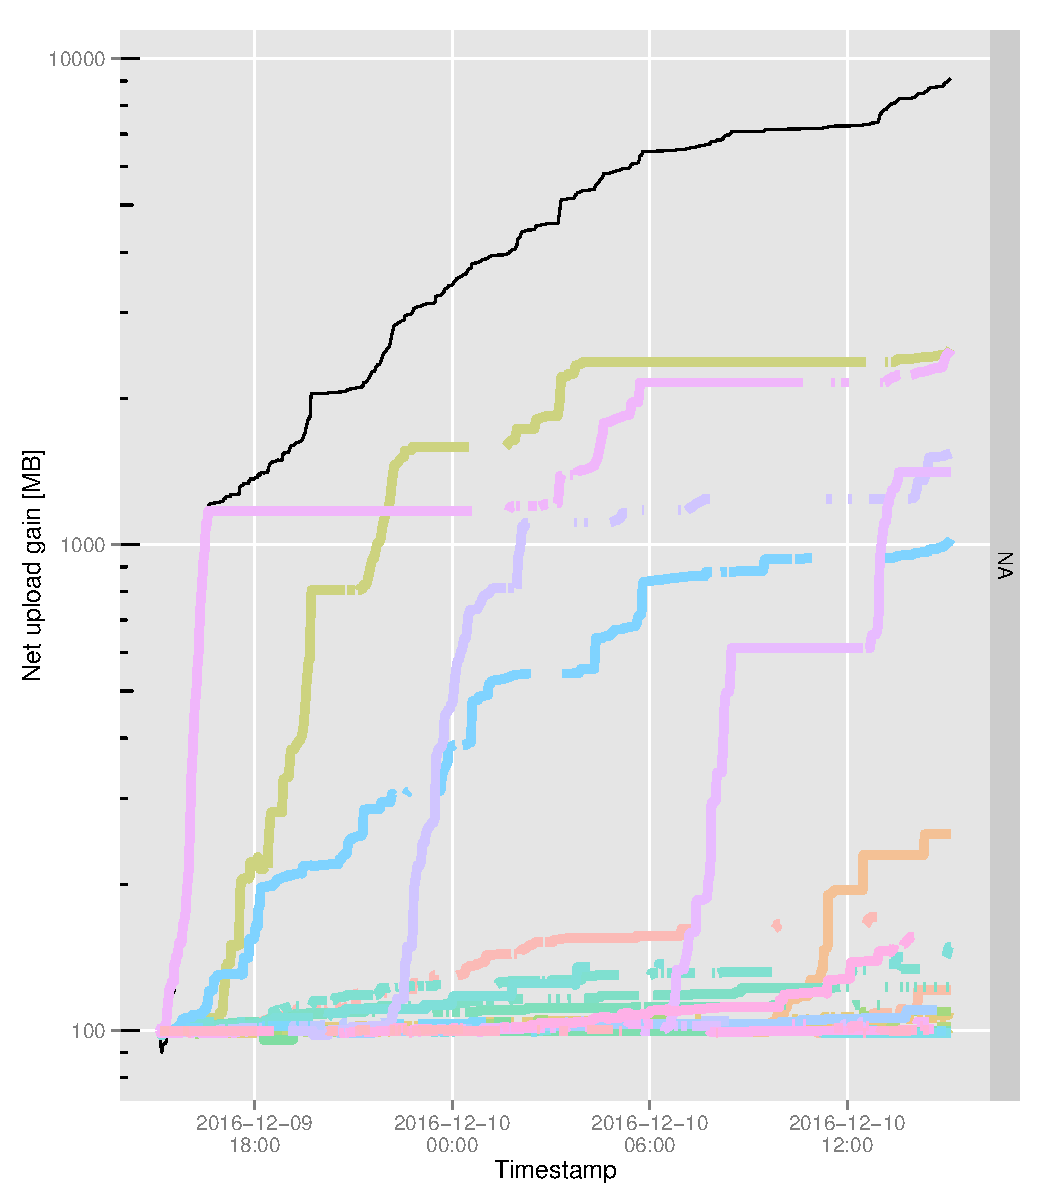
\includegraphics[width=\textwidth]{pics/results/m138.pdf}
			\caption{24 hour old experiment}
		\end{subfigure}
		\caption{New vs old experiments (run separately) result on 24 hour}
	\end{adjustwidth}
\end{figure}

\begin{figure}[t!]
	\begin{adjustwidth}{-2.5cm}{}
		\begin{subfigure}[t]{0.7\textwidth}
			\centering
			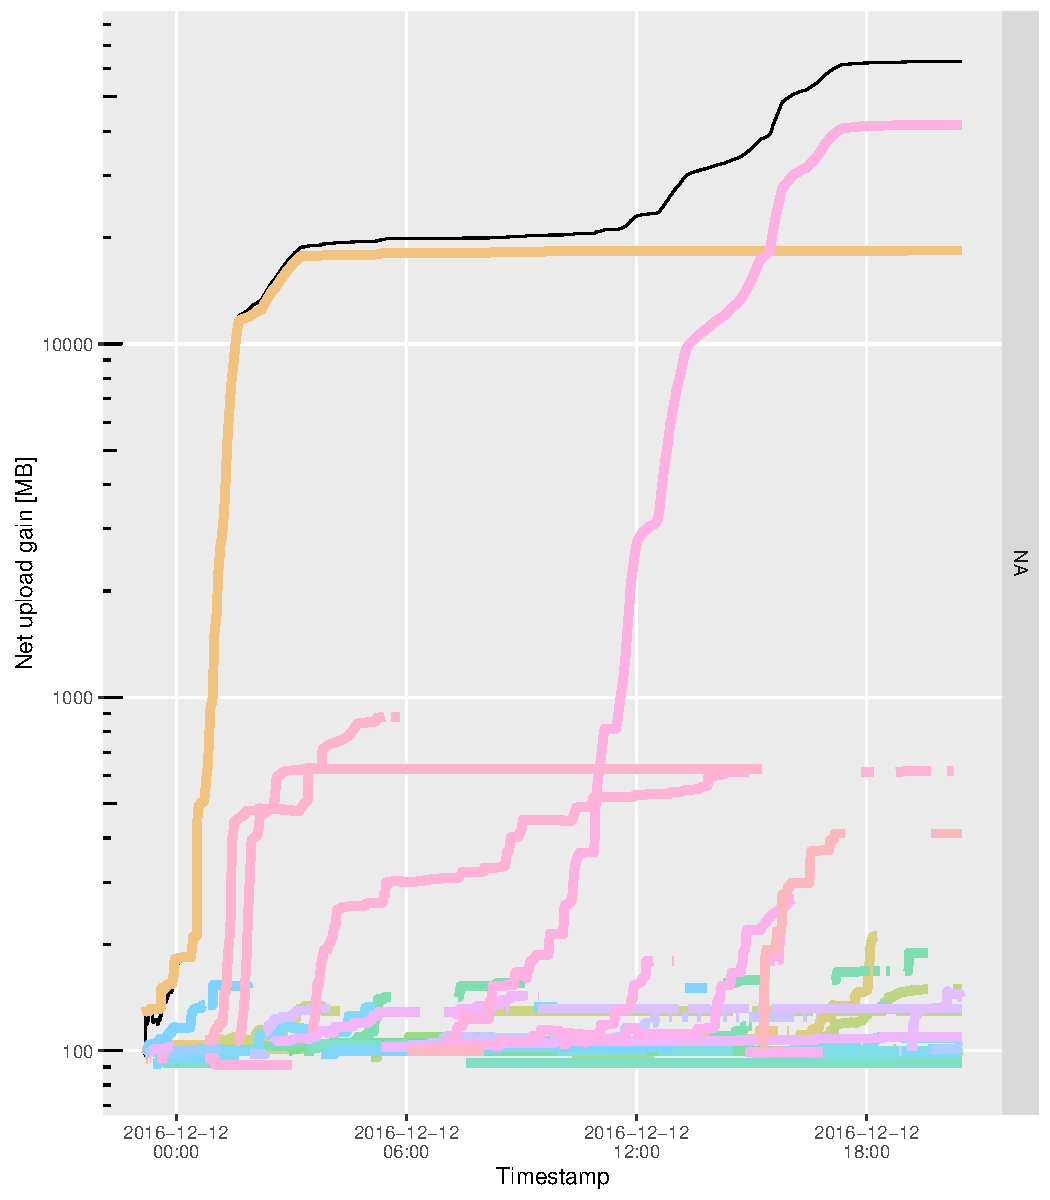
\includegraphics[width=\textwidth]{pics/results/b137.pdf}
			\caption{24 hour new experiment.}
		\end{subfigure}
		~
		\begin{subfigure}[t]{0.7\textwidth}
			\centering
			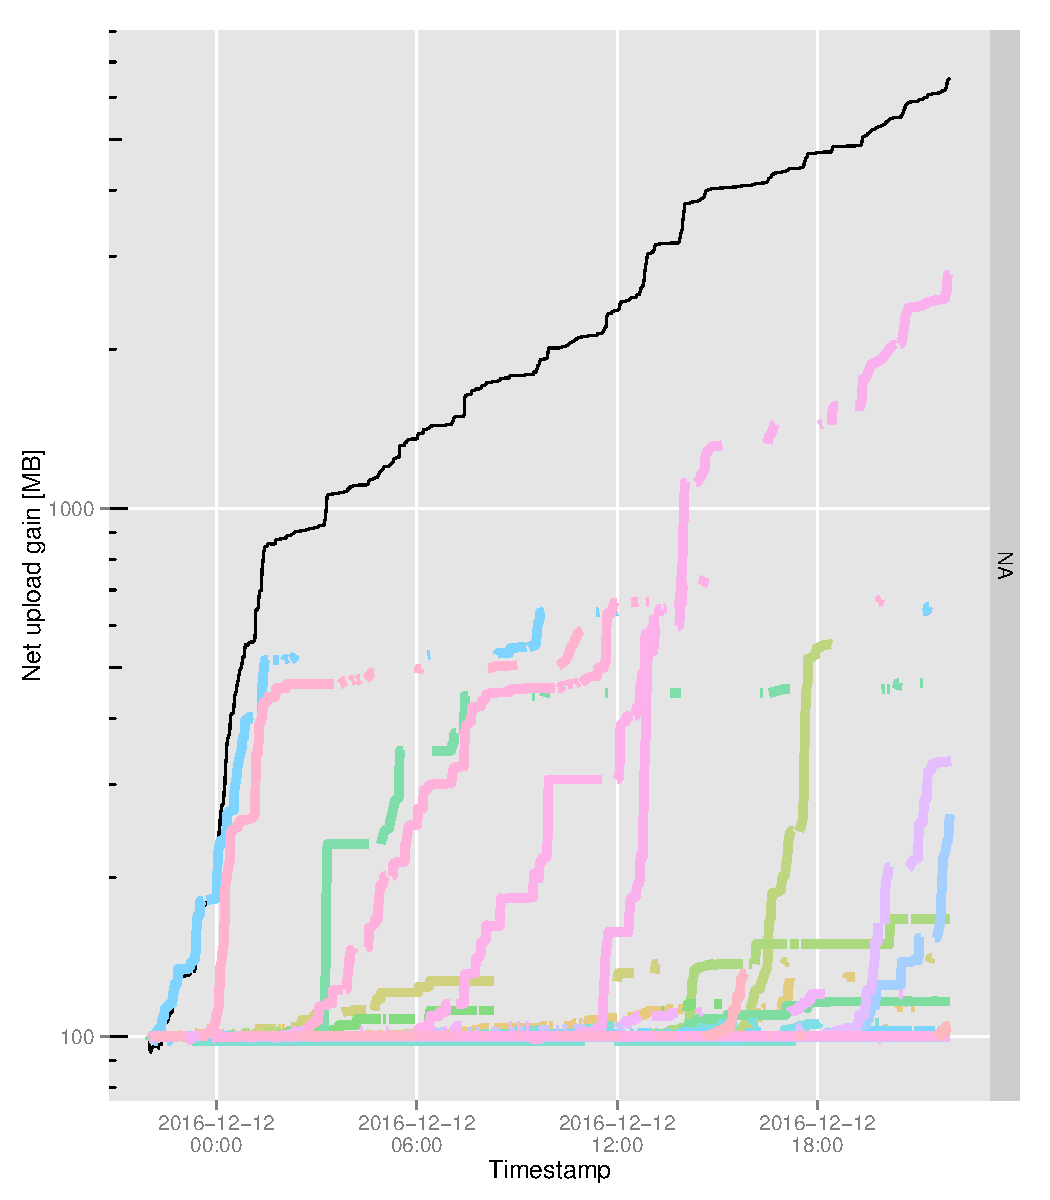
\includegraphics[width=\textwidth]{pics/results/m139.pdf}
			\caption{24 hour old experiment}
		\end{subfigure}
		\caption{New vs old experiments (run in parallel) result on 24 hour}
	\end{adjustwidth}
\end{figure}
%\begin{itemize}
%	\item old one use \textit{net upload gain}. etree.org for two day (48 hour). Test with 1 and half day.
%	\item Best old one is SeederRatio with 5 minute with 1 ratio (gain higher upload gain). Optimal : 3 ratio.
%	\item CM+boost : seederratio, 5 minutes, 3 ratio
%	\item mihai 136 12 hour. runs first. 6dec
%	\item cm 133. 12 hour. runs second. 8dec
%	\item mihai 137, cm 134 : 12 hour. In parallel
%	\item mihai 138 -> cm 136 24h
%	\item mihai 139 & 137 24h par
%\end{itemize}

\section{Priority}
% #50 -> 25k secs : 7 hour
% #50 -> 12h : 
\todo[inline]{temporary graph}
\begin{figure}[h]
	\centering
	\includegraphics[width=\textwidth]{pics/results/tmp_prio_4.png}
	\caption{Download speed of user download activity vs credit mining}
	\label{fig:cmpriomeanagg}
\end{figure}
\begin{figure}[h]
	\centering
	\includegraphics[width=\textwidth]{pics/results/tmp_prio_5.png}
	\caption{Download speed of user download activity only}
	\label{fig:cmpriomean}
\end{figure}
\section{Swarm performance}
\begin{figure}[h]
	\centering
	\includegraphics[width=\textwidth]{pics/results/tmp_cm.png}
	\caption{Swarm performance with credit mining}
	\label{fig:swarmcmperf}
\end{figure}

\begin{figure}[h]
	\centering
	\includegraphics[width=\textwidth]{pics/results/tmp_nocm.png}
	\caption{Swarm performance without credit mining}
	\label{fig:swarmnocmperfrecent}
\end{figure}